\chapter{Amazon Web Services (AWS)}

Amazon usluge za web (engl. \textit{Amazon Web Services} - AWS) sveobuhvatna je platforma za računarstvo u oblaku koju pruža Amazon te sadrži brojne usluge u oblaku, uključujući infrastrukturu (engl. \textit{Infrastructure as a Service} - IaaS), platformu (engl. \textit{Platform as a Service} - PaaS) i softver (engl. \textit{Software as a Service} - SaaS). AWS usluge nude organizacijske alate kao što su računalna snaga, baza podataka i usluge isporuke sadržaja \cite{what_is_aws}. 

AWS je podijeljen u više različitih usluga koje se mogu pojedinačno konfigurirati na temelju korisnikovih potreba. Neke od usluga koje nudi AWS su: pohrana, baze podataka, migracija, povezivanje, monitoriranje, sigurnost, analitika, umjetna inteligencija te razvoj mobilnih aplikacija. 

AWS pruža usluge iz mnogo podatkovnih centara (engl. \textit{data center} - DC) koji su raspodijeljeni po zonama dostupnosti (engl. \textit{availability zone} - AZ) diljem regija cijelog svijeta. Jedna regija obuhvaća nekoliko fizički bliskih zona povezanih mrežom niske latencije. 

Također, nude se brojne mogućnosti za razvojne inženjere u sklopu AWS-a. Nudi alate naredbenog retka (engl. \textit{command-line tools}) i pakete za razvoj programa (engl. \textit{Software Development Kit} - SDK) za puštanje aplikacija u produkciju (engl. \textit{deployment}) i upravljanje vlastitim uslugama i aplikacijama. Paketi za razvoj programa dostupni su u raznim programskim jezicima, uključujući programske jezike C++, Android, iOS, Java, Node.js, Python i Ruby.
 
\section{Usluge AWS-a za IoT sustave}

AWS isto tako nudi brojne usluge za razvoj IoT sustava. Usluga AWS-a za IoT pruža platformu za upravljanje IoT uređajima te obradu podataka i njihovu pohranu na druge AWS usluge, poput baze podataka. AWS IoT pruža usluge u oblaku koje povezuju IoT uređaje s drugim uređajima i uslugama AWS-a u oblaku. Također pruža software za uređaje, poput paketa za razvoj programa, za jednostavniju integraciju s uslugama AWS-a za IoT. Na slici \ref{fig:aws_iot_arch} nalazi se prikaz arhitekture usluga koje AWS nudi za razvoj IoT sustava.

\begin{figure}[ht]
	\centering
	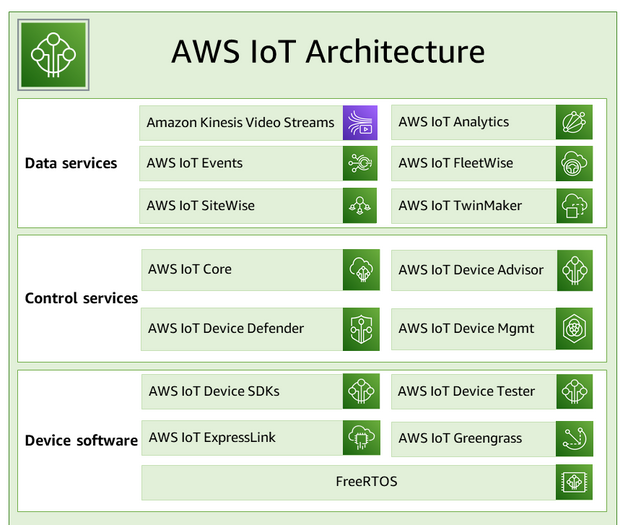
\includegraphics[scale=0.8]{imgs/aws_iot_arch}
	\caption{Arhitektura usluga AWS-a za IoT \cite{aws_docs}}
	\label{fig:aws_iot_arch}
\end{figure}

AWS IoT podržava sljedeće komunikacijske protokole:
\begin{itemize}
	\item MQTT (engl. \textit{Message Queuing Telemetry Transport}),
	\item HTTPS,
	\item LoRaWAN (engl. \textit{Long Range Wide Area Network}),
	\item TLS.
\end{itemize}

U nastavku su opisane usluge za razvoj IoT sustava u sklopu AWS-a.

\subsection{AWS IoT Core}

AWS IoT Core ključna je komponenta za integraciju oblaka i fizičkih uređaja. Omogućava povezivanje uređaja i preusmjeravanje poruka na usluge AWS-a. Koristi MQTT koji je standardni protokol za razmjenu poruka u IoT sustavima. To je lagan (engl. \textit{lightweight}) protokol za prijenos poruka temeljen na objavi/pretplati sustavu, te je pogodan za povezivanje udaljenih uređaja uz minimalnu potrošnju \cite{what_is_mqtt}. AWS IoT Core pruža paletu značajki za razmjenu poruka temeljenih na protokolu MQTT, koje pomažu pri izradi prilagodljive i skalabilne IoT arhitekture \cite{aws_docs}. Na slici \ref{fig:aws_iot_core_overview} nalazi se pregled rada usluge AWS IoT Core.

\begin{figure}[ht]
	\centering
	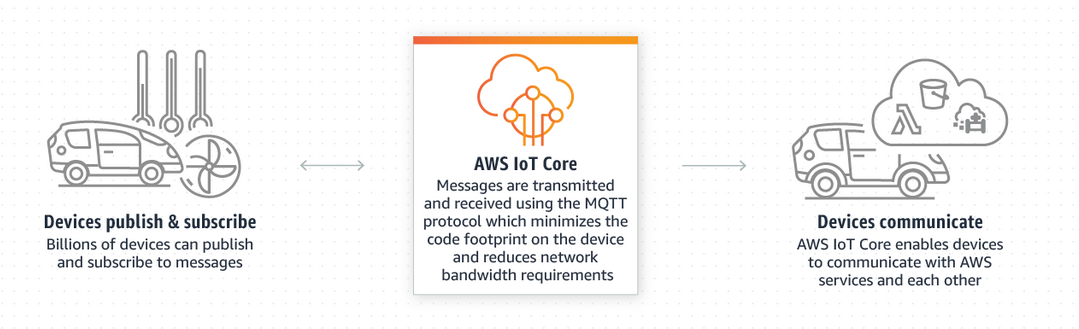
\includegraphics[scale=0.6]{imgs/aws_iot_core_overview}
	\caption{Princip rada usluge AWS IoT Core \cite{aws_docs}}
	\label{fig:aws_iot_core_overview}
\end{figure}

AWS IoT Core pruža usluge koje povezuju oblak AWS-a s IoT uređajima kako bi se ostale usluge u oblaku i aplikacije mogle međusobno komunicirati s tim uređajima. Na slici \ref{fig:aws_iot_core_components} nalaze se svi segmenti usluge AWS IoT Core te kako oni komuniciraju s vanjskim dijelovima. Zelenom bojom označena je sama usluga, narančastom bojom fizički uređaji, odnosno stvari (engl. \textit{Things}), sivom bojom druge IoT aplikacije unutar AWS-a, dok su plavom bojom označene ostale usluge koje se nude u ekosustavu AWS.

\begin{figure}[ht]
	\centering
	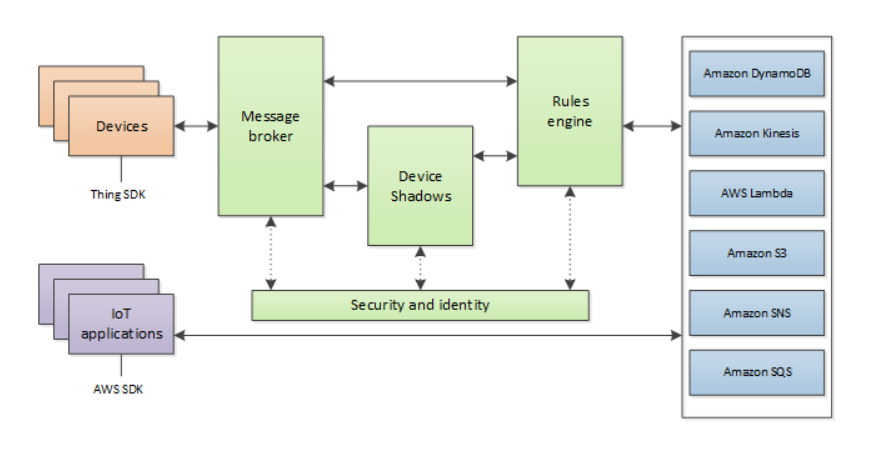
\includegraphics[scale=0.6]{imgs/aws_iot_core_components}
	\caption{Komponente usluge AWS IoT Core \cite{aws_docs}}
	\label{fig:aws_iot_core_components}
\end{figure}

U nastavku su navedene ključne usluge koje pokriva AWS IoT Core.

\subsubsection{Usluge za slanje poruka}

AWS IoT Core usluge za povezivanje pružaju sigurnu komunikaciju s IoT uređajima i upravlja porukama koje prolaze između uređaja i oblaka.

Prilazni uređaj omogućuje uređajima sigurnu i efikasnu komunikaciju sa sustavom AWS. Komunikacija je osigurana sigurnosnim protokolima koji koriste  X.509 certifikate. 

Broker za poruke pruža mehanizam uređajima i aplikacijama slanje i primanje poruka. Moguće je koristiti protokol MQTT ili direktno WebSocket za objavu i pretplatu na teme. Uređaji i klijenti koriste HTTP REST sučelje za objavu poruka brokeru. Broker zatim distribuira podatke na uređaje koji su se pretplatili na određene teme kao i na druge AWS aplikacije te usluge koje prate teme na brokeru.

AWS IoT Core za protokol LoRaWAN omogućava postavljanje privatne LoRaWAN mreže tako što poveže LoRaWAN te prilazne uređaje na AWS bez potrebe za razvojem mrežnog servera za LoRaWAN (engl. \textit{LoRaWAN Network Server} - LNS). Poruke primljene od LoRaWAN uređaja šalju se na stroj za pravila (engl. \textit{rules engine}) gdje se formatiraju i prosljeđuju ostalim AWS uslugama.

Stroj za pravila povezuje podatke iz brokera s drugim AWS IoT uslugama za pohranu i dodatnu obradu. Primjerice, moguće je umetati ili pretraživati po podatkovnim tablicama ili pozvati određene definirane funkcije na temelju izraza definiranog u stroju. Isto tako, moguće je obraditi te podatke i proslijediti novostvoreni format poruka drugim uslugama ili bazama podataka.

\subsubsection{Upravljačke usluge}

Upravljačke usluge AWS IoT Core komponente pružaju sigurnost uređaja te značajke za upravljanje i registraciju novih uređaja.

Moguće je definirati vlastite autorizatore radi upravljanja autentifikacijskim i autorizacijskim strategijama koristeći vlastiti servis za autentifikaciju i Lambda funkcije za računanje koje AWS nudi. 

Usluga za postavljanje (engl. \textit{provisioning}) uređaja omogućava konfiguriranje i prijavu uređaja u AWS koristeći predložak koji opisuje resurse potrebne uređaju: \textit{stvar}, certifikat i nekoliko politika. \textit{Stvar} je unos u registar koji sadrži atribute opisa uređaja. Uređaji koriste certifikate za autentifikaciju s AWS IoT sustavom. Politike određuju koje operacije uređaj može izvršiti. 

Isto tako, moguće je definirati grupe za lakšu kategorizaciju i upravljanje uređajima. Grupe također mogu imati podgrupe, i tako graditi hijerarhiju grupa. Sve akcije izvršene na roditeljima propagiraju se do najdubljih podgrupa. Dozvole dodijeljene grupi primjenjuju se na sve uređaje u toj grupi i svim njihovim podgrupama. 

Usluga za poslove (engl. \textit{jobs}) omogućava definiranje udaljenih operacija koje se pošalju i izvrše na fizičkim uređajima spojenih u oblak. Posao se može odnositi preuzimanje i instalaciju aplikacija, ažuriranje sustava, ponovno pokretanje, obnova certifikata i slično.

Registar organizira resurse pridružene uređajima u oblaku. Moguće je registrirati uređaje i pridružiti im maksimalno po tri atributa. Isto tako, uređajima se mogu pridružiti certifikati i klijentski ID za MQTT komunikaciju kako bi se olakšalo otklanjanje budućih grešaka.

Usluga za sigurnost i identitet pruža dijeljenu odgovornost za sigurnost unutar AWS oblaka. Fizički uređaji moraju držati vjerodajnice na sigurnom kako bi se podaci mogli slati brokeru na siguran način. Značajke za sigurnost koriste i stroj za pravila kao i broker za poruke radi sigurnog prijenosa podataka drugim uslugama unutar AWS ekosustava.

\subsubsection{Usluge za uređaje}

AWS IoT Core osigurava pouzdano aplikacijsko iskustvo iako uređaji nisu uvijek povezani. 

Sjena uređaja (engl. \textit{Device Shadow}) dokument je u JSON formatu koji se koristi za pohranu i dohvat trenutnog stanja i informacija o uređaju. AWS nudi uslugu koja održava stanje uređaja (engl. \textit{Device Shadow service}) kako bi aplikacije mogle komunicirati s uređajem bez obzira je li uređaj na mreži ili ne. Kada uređaj nije priključen na mrežu, usluga sjene uređaja upravlja podacima za povezane uređaje. Kada se uređaj ponovno spoji na mrežu, sinkronizira stanje sa sjenom uređaja koja se nalazi u oblaku. Uređaji također mogu objavi svoje stanje usluzi u bilo kojem trenutku kako bi bilo na raspolaganju drugim aplikacijama i uređajima. 

\subsection{AWS IoT OTA}

\subsection{AWS IoT Device Shadow}

\subsection{AWS IoT Jobs}

\subsection{AWS IoT Device Defender}

\subsection{AWS IoT Fleet Provisioning}

\subsection{Ostale dostupne IoT usluge u sustavu AWS}

Uz ranije opisanu glavnu komponentu IoT Core koju nudi AWS za stvaranje IoT aplikacija, u samom ekosustavu nalazi se još mogućnosti za jednostavniju integraciju oblaka i fizičkih uređaja. U nastavku su ukratko opisane ostale usluge koje se mogu integrirati uz jezgrenu uslugu AWS IoT Core.

Važno je napomenuti kako nisu sve usluge dostupne u svim regijama unutar platforme AWS.

\subsubsection{IoT Analytics}

AWS IoT Analytics automatizira korake potrebne za analizu podataka prikupljenih od IoT uređajima. Filtrira, transformira i obogaćuje podatke prije nego ih pohrani u vremensku bazu podataka za daljnju analizu. Moguće je postaviti uslugu da prikuplja podatke s uređaja samo koji su potrebni, vrši matematičke operacije i dopunjava podatke raznim metapodacima, primjerice o lokaciji. Zatim se podaci mogu analizirati koristeći ugrađeni sustav za pretraživanje koji koristi SQL sintaksu ili pak vršiti kompleksniju analizu koristeći usluge umjetne inteligencije. Isto tako, ova usluga nudi vizualizaciju podataka integracijom s dodatnom uslugom Amazon QuickSight. 

\subsubsection{IoT Device Defender}

AWS IoT Device Defender potpuna je usluga koja pomaže pri osiguranju IoT uređaja. Kontinuirano revidira IoT konfiguracije radi provjere jesu li sve u skladu s najboljim sigurnosnim praksama. Također pruža kontinuirano monitoriranje sigurnosnih metrika s uređaja i AWS IoT Core kako bi se detektirale anomalije u ponašanju pojedinih uređaja. 

Ova usluga također omogućuje slanje alarma na konzolu AWS IoT sustava i na uslugu za monitoriranje Amazon CloudWatch. Koriste se ugrađene mitigacijske akcije kako bi se izolirali nesigurni uređaji.

\subsubsection{IoT Events}

AWS IoT Events usluga služi za praćenje događaja u sustavu. Ova usluga prati ulazne podatke s više IoT uređaja i aplikacija radi prepoznavanja uzoraka i pokretanja prikladnih operacija na određene događaje. Moguće je pratiti ne samo fizičke uređaje, nego i druge AWS aplikacije integrirane u IoT sustav.

\subsubsection{IoT FleetWise}

AWS IoT FleetWise jest usluga koja se koristi za prikupljanje podataka od vozila i njihovu organizaciju u oblaku. Prikupljeni se podaci mogu koristiti za poboljšanje kvalitete, performansa i autonomije vozila. Također podržava više različitih protokola i podatkovnih formata. Ova usluga pomaže pri transformaciji \textit{low-level} poruka u oblik čitljiv čovjeku i standardizira podatke radi lakše analize u oblaku. Moguće je također definirati vrstu podataka i trenutak u kojem se ti podaci šalju u oblak.

Kada su podaci o vozilu u oblaku, mogu se koristiti u aplikacijama koje analiziraju zdravlje vozila. Ove informacije mogu pomoći pri identifikaciji potencijalnih problema u održavanju i pri unapređenju naprednih tehnologija poput autonomne i asistirane vožnje integracijom strojnog učenja.

\subsubsection{IoT Greengrass}

AWS IoT Greengrass jest usluga otvorenog koda (engl. \textit{open source}) za računarstvo na rubu (engl. \textit{edge computing}) i u oblaku koja pomaže pri izradi, objavi i upravljanju IoT aplikacija na uređajima. Može se koristiti za omogućavanje uređajima lokalno reagiranje na podatke koje generiraju, pokretanje modela strojnog učenja za predikciju, te filtriranje i agregaciju podataka s uređaja. Omogućava uređajima da prikupljaju i analiziraju podatke ne u oblaku, nego ili na samom uređaju ili drugom mjestu koje je bliže izvorištu tih podataka. Također može komunicirati na siguran način s uslugom AWS IoT Core i izvoziti podatke u oblak. Karakteristika računarstva u rubu, koje omogućava ova komponenta, jest približavanje računanja izvorišnim uređajima, čime se poboljšava vrijeme odziva i štedi propusnost \cite{what_is_edge}.

\subsubsection{IoT Roborunner}

AWS IoT RoboRunner nova je usluga koja pruža infrastrukturu za optimizaciju robota iz jedne točke gledišta. Uz pomoć ove usluge moguće je izgraditi aplikacije za jednostavniji međusobni rad robota. Namijenjena je za industrijske robote i automatizirane sustave za olakšano upravljanje opremom. Pruža centralne repozitorije podataka za pohranu te podržava različite podatkovne formate od raznih robota i autonomnih sustava.

\subsubsection{IoT TwinMaker}

AWS IoT TwinMaker usluga je za kreiranje operativnih digitalnih dvojnika fizičkih i digitalnih sustava. Stvara digitalne vizualizacije koristeći mjerenja i analize iz raznih senzora i kamera radi praćenja stvarnog stanja i uvjeta u kojima se objekt, zgrada ili kompleks nalazi. Podaci iz stvarnog svijeta se mogu koristiti za dijagnostiku i ispravljanje pogrešaka ili pak optimizaciju operacija. 

Digitalni dvojnik (engl. \textit{digital twin}) digitalna je reprezentacija sustava i svih njegovih fizičkih i digitalnih komponenti. Dinamički se ažurira primitkom novih podataka kako bi simulirao stvarno stanje i ponašanje sustava. 


\subsubsection{IoT SiteWise}

AWS IoT SiteWise jest usluga koja skalabilno prikuplja, modelira, analizira i vizualizira podatke iz industrijske opreme. Usluga pruža kreiranje web aplikacija za operativne korisnike radi prikaza i analize industrijskih podataka u stvarnom vremenu. Moguće je dobiti uvide u podatke i operacije konfiguriranjem i praćenjem raznih metrika, primjerice efektivnost i efikasnost opreme. Ovu je uslugu moguće koristiti jedino uz ranije opisan IoT TwinMaker.

\eject